\documentclass[a4paper,12pt]{article}
 \usepackage[italian]{babel} 
\usepackage{graphicx}
\usepackage{caption}
\usepackage{geometry}
\usepackage{enumitem}
\usepackage{fancyhdr}
\usepackage{svg-extract}
\usepackage{hyperref}
\geometry{a4paper, top=1.5cm, bottom=1.5cm, left=1.5cm, right=1.5cm, }
\setlength{\parindent}{0pt} %\setlength{\parskip}{0,25cm plus1mm minus1mm}
\graphicspath{ {/Users/nicola/Documents/GitHub/lifemanager/images/Latex/} } 
\lhead{
\includegraphics[width=5cm]{logounitn.jpg}}
\rhead{
\includegraphics[width=3cm]{logolifemanager.png}}
\setlist[itemize]{leftmargin=5.5mm}




%\fancyhead[L]{
\includegraphics[width=5cm]{logounitn.jpg}}
\renewcommand{\headrulewidth}{0pt}
\raggedbottom

%-----------------------------------------
 \title{LifeManager}
 \author{
 Corso di Ingegneria del software\\ \\Luca Boschiero, Mauro Meneghello, Nicola Turniano
 }
 \begin{document} 
 \maketitle
 \thispagestyle{fancy}
 %-----------------------------------------
 


 %-----------------------------------------


\section*{Dominio e obiettivi del progetto}
Questo progetto ha come obiettivo lo sviluppo di una WebApp per gestire i vari aspetti relativi alla vita quotidiana di una persona. 

L'applicazione, denominata {\scshape LifeManager}, infatti permetterà ad un individuo di semplificare molti aspetti della propria routine, organizzando e gestendo attività quotidiane, cose da fare, informazioni e denaro. 

Questa semplificazione si basa sull'esigenza di avere tutto ciò racchiuso in un unico servizio e facilmente accessibile in ogni momento della giornata, differenziandosi dalle applicazioni presenti attualmente sul mercato.

Più in dettaglio, il sistema deve essere in grado di:


\begin{itemize}
 \setlength\itemsep{0.01em}

\item {\sffamily  Gestire registrazione e autenticazione di un individuo } 
\\Il sistema permette ad un utente di registrarsi e, dopo aver effettuato l'accesso, di procedere all'utilizzo dell'applicativo
\item {\sffamily Gestire del budget personale } 
\\Il software permette all'utente di gestisce le proprie entrate e le uscite, aggiungendo o rimuovendo movimenti di denaro, organizzandoli secondo categorie, visualizzando statistiche sui propri pagamenti, ricercando una spesa precisa consentendo così di monitorare i propri movimenti.
\item {\sffamily Gestire gli eventi } 
\\L'utente visualizza un calendario in cui può aggiungere eventi o promemoria e gestirli in modo personalizzato, impostando avvisi che verranno ricevuti in prossimità degli appuntamenti.
\item {\sffamily  Gestire le liste di interesse} 
\\ Il sistema permette all'utente di creare e organizzare varie liste le cui voci si possono contrassegnare attraverso delle checkbox. Alcune liste sono già pre impostate: lista della spesa e la to-do List.
\item {\sffamily Gestire i luoghi di interesse } 
\\Il sistema permette all'utente di cercare dei luoghi particolari visualizzandone le informazioni attraverso una mappa e salvarli come preferiti, visitati o da visitare, aggiungendo anche note e categorie, e cercare tra di essi.
\item {\sffamily Gestire le carte fedeltà } 
\\L'utente inserisce le proprie carte fedeltà fornite dai negozi e, quando necessario, visualizza il codice a barre facilmente scannerizzabile.
\item {\sffamily Gestire le ricette} 
\\ Il sistema permette all'utente di scrivere e memorizzare ricette specificandone tutti i dettagli, ingredienti e procedimento, e aggiungere facilmente tutti o alcuni degli ingredienti della ricetta alla propria lista della spesa.

\end{itemize}

\section*{Attori}
\begin{itemize}
 \setlength\itemsep{0.01em}
\item {\sffamily  Utenti}
\\ Utenti autenticati e utenti non autenticati
\item {\sffamily  Servizi interni}
\\ LifeManager services
\item {\sffamily  Servizi esterni}
\\ Servizi di autenticazione, notifiche via mail, geolocalizzazione, mappe, calendario, traduttore di codici a barre

\begin{center}
  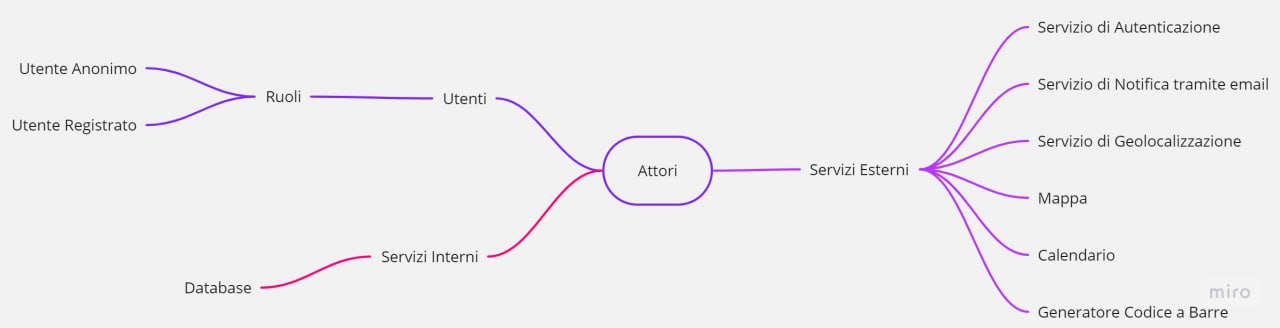
\includegraphics[width=13cm]{mind_map.jpeg}
  \captionof{figure}{Mind map attori}
\end{center}

\end{itemize}
Per una descrizione più dettagliata degli attori, fare riferimento alla Mind Map e alla descrizione riportata nella sezione dell'Analisi di contesto.

\section*{Analisi SWOT}
{\sffamily  Punti di forza}
\begin{itemize} \setlength\itemsep{0.01em}
\item Interesse da parte del pubblico a causa della mancanza di un'unica applicazione di questo tipo.
\item Aumenta l'organizzazione e permette di risparmiare tempo.
\item User interface facile e intuitiva che facilita l'organizzazione.
\item Avere tutto insieme.
\item Migliorare le abitudini e la routine quotidiana grazie a promemoria e avvisi.
\end{itemize}

{\sffamily  Punti di debolezza}
\begin{itemize} \setlength\itemsep{0.01em}
\item Molte persone potrebbero preferire i metodi "classici", non aprendosi al "nuovo".
\item Template troppo rigidi (alle persone potrebbe non andare bene come vengono organizzati i propri dati).
\item Funzionalità già esistenti nel telefono (ma non congiuntamente).
\item Mancanza di esperienza del team.
\item Alcune fasce di età (over 60) sono poco propense alla digitalizzazione e informatizzazione.
\end{itemize}

{\sffamily  Opportunità}
\begin{itemize} \setlength\itemsep{0.01em}

\item Espansione da uno a più individui sincronizzati per gestire famiglie e/o gruppi.
\item Aumento delle persone che potrebbe essere interessate conseguentemente al maggiore utilizzo delle tecnologie e di Internet.
\item Statistiche che permettono all'utente di prendere atto delle proprie abitudini.
\end{itemize}

{\sffamily  Minacce}
\begin{itemize} \setlength\itemsep{0.01em}

\item Possibile concorrenza.
\item Possibile assenza di Internet.
\item Possibile dipendenza dal sistema, che porta al dimenticarsi di come si faceva prima.
\item Errori o malfunzionamenti dell'app che potrebbero compromettere l'utilizzo e causare malcontento.
\end{itemize}

\newpage
\section*{User stories}
\begin{itemize} \setlength\itemsep{0.01em}
\item \textbf {US1} Come utente non registrato (anonimo), voglio potermi registrare al sistema inserendo: nome, cognome, username, email e password, in modo da poter accedere all'applicazione. É inoltre accettata la registrazione tramite Google. (\hyperlink{RF1}{RF1}, \hyperlink{RNF1}{RNF1})

\begin{center}
 \fbox{ 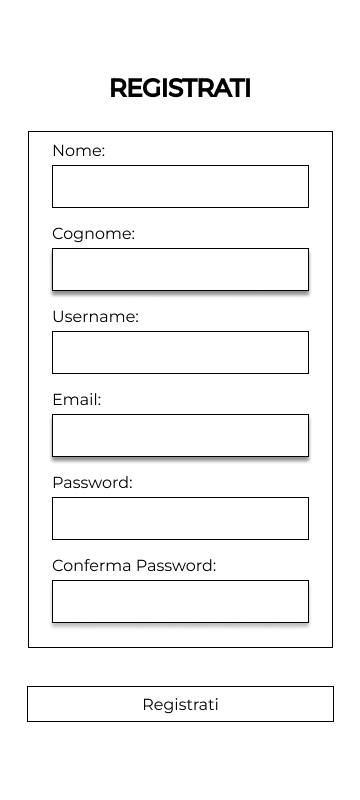
\includegraphics[width=2.4cm]{Registrazione.png}}
\end{center}

\item\textbf {US2} Come utente registrato, voglio poter accedere inserendo le mie credenziali: username o email e password oppure tramite Google, in modo da poter utilizzare le funzionalità dell'applicazione. Se dimentico la password voglio poterla recuperare facilmente ricevendo una mail e resettando la password. (\hyperlink{RF2}{RF2},\hyperlink{RNF1}{RNF1}, \hyperlink{RNF2}{RNF2}, \hyperlink{RNF3}{RNF3})

\begin{center}
  \fbox{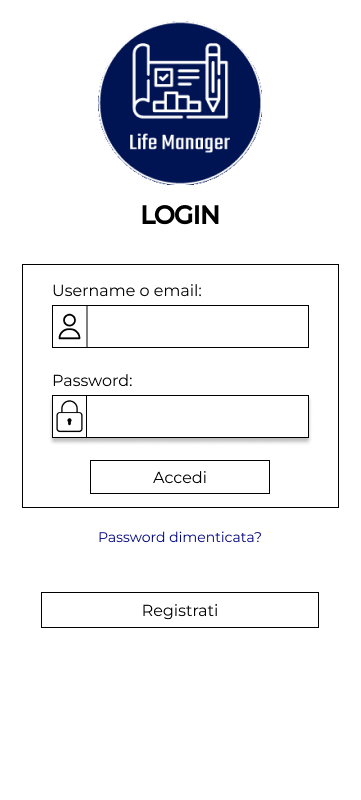
\includegraphics[width=2.4cm]{Login.png}}
\end{center}


\item \textbf {US3} Come utente autenticato, voglio poter visualizzare tutte le funzionalità nella home page sotto forma di menù iniziale, e cliccando sull'icona di ogni funzionalità accedere alla scheda corrispondente, in modo da poter accedere alle task in modo semplice ed intuitivo. Inoltre dalla home page voglio avere due icone che mi permettono di entrare nella scheda impostazioni e in quella profilo in modo da poterle visualizzare e gestire facilmente. (\hyperlink{RF3}{RF3}, \hyperlink{RF4}{RF4}, \hyperlink{RF30}{RF30}, \hyperlink{RF31}{RF31})

\begin{center}
  \fbox{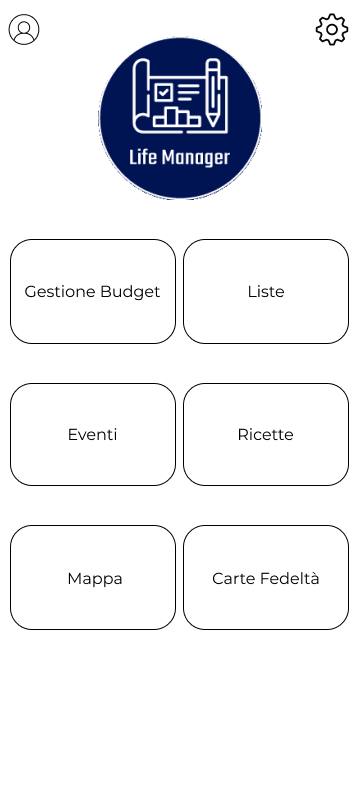
\includegraphics[width=2.4cm]{Home Page.png}}
  \fbox{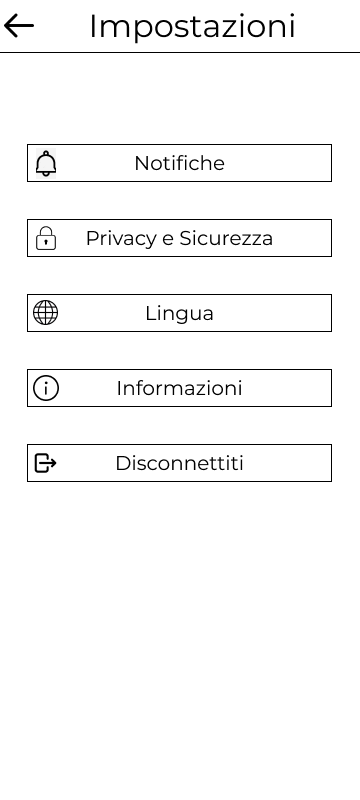
\includegraphics[width=2.4cm]{Impostazioni.png}}
  \fbox{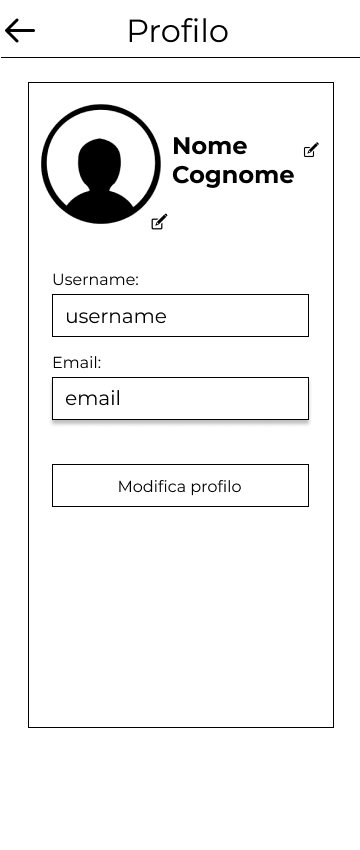
\includegraphics[width=2.4cm]{Account.png}}
\end{center}

\item \textbf {US4} Come utente autenticato, voglio poter aggiungere o rimuovere le mie entrate e uscite, visualizzare il saldo totale e ricercare una o un insieme di spese, in modo da tenere sotto controllo tutti i miei movimenti e visualizzare il saldo aggiornato. Inoltre voglio poter creare e accedere in modo veloce alle categorie in cui i movimenti sono classificati attraverso un bottone, in modo da visualizzare e gestire i movimenti categoria per categoria. (\hyperlink{RF5}{RF5}, \hyperlink{RF6}{RF6},\hyperlink{RF7}{RF7},\hyperlink{RF8}{RF8},\hyperlink{RF9}{RF9})

\begin{center}
  \fbox{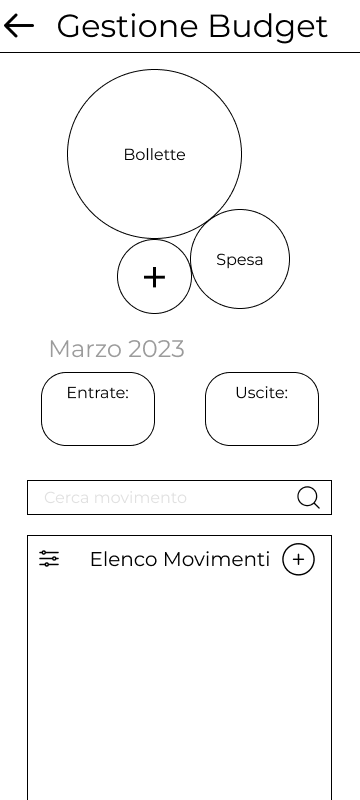
\includegraphics[width=2.4cm]{Gestione Budget.png}}
  \fbox{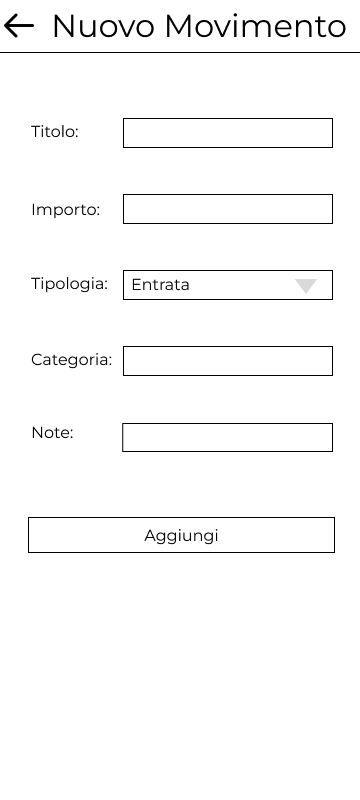
\includegraphics[width=2.4cm]{Aggiungi Movimento.png}}
  \fbox{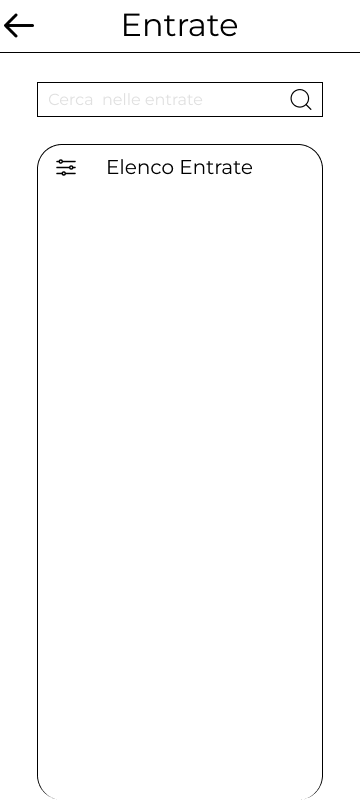
\includegraphics[width=2.4cm]{Elenco Entrate.png}}
  \fbox{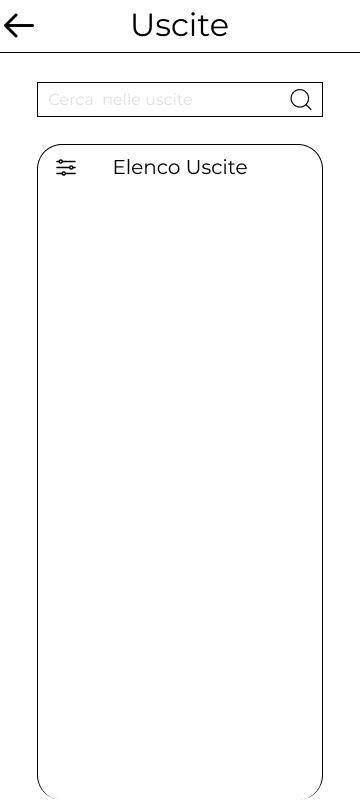
\includegraphics[width=2.4cm]{Elenco Uscite.png}}
  \fbox{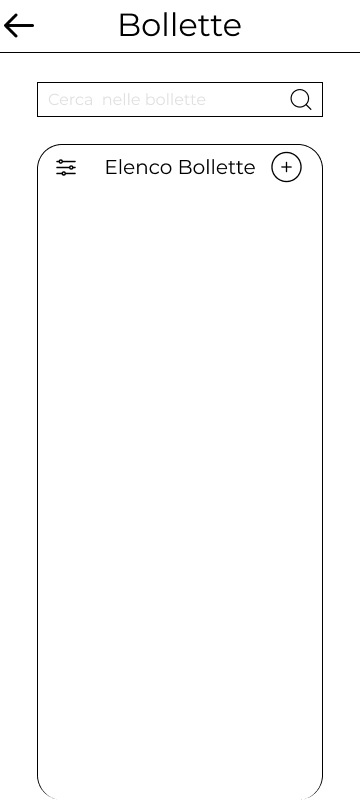
\includegraphics[width=2.4cm]{Elenco Bollette.png}}
  \fbox{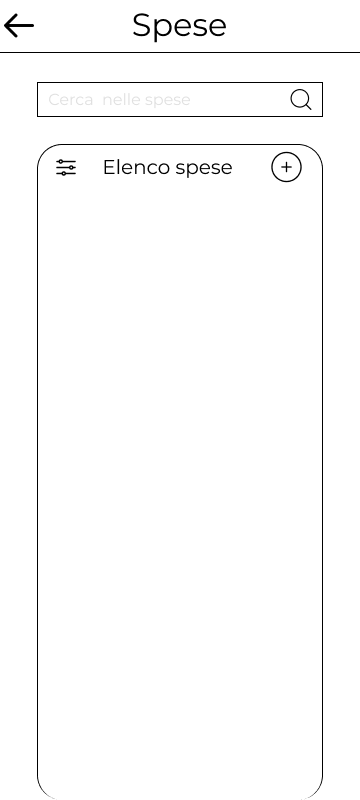
\includegraphics[width=2.4cm]{espese.png}}
  \fbox{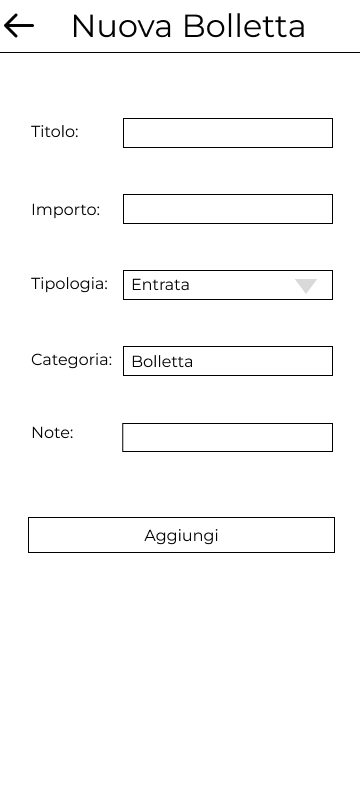
\includegraphics[width=2.4cm]{Aggiungi Bolletta.png}}
  \fbox{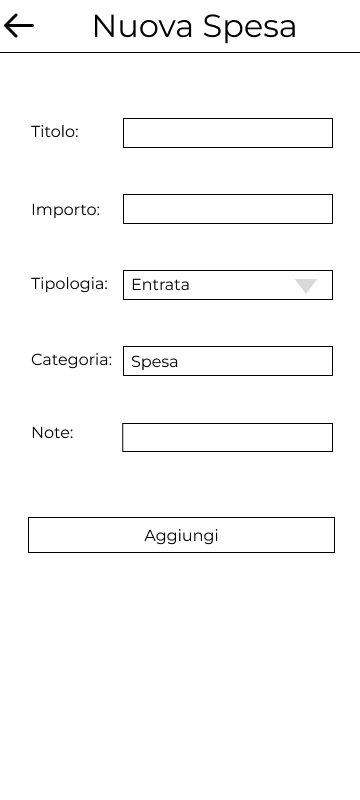
\includegraphics[width=2.4cm]{aspesa.png}}
  \fbox{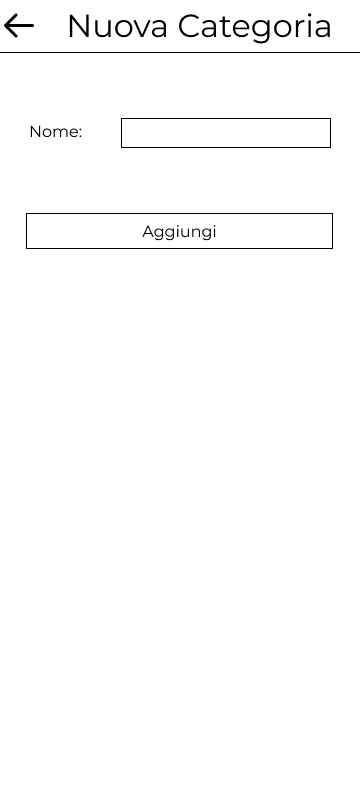
\includegraphics[width=2.4cm]{Aggiungi Categoria.png} }
\end{center}

\newpage

\item \textbf {US5}  Come utente autenticato, voglio poter visualizzare un calendario in cui posso aggiungere, rimuovere, modificare eventi. Voglio anche che, su richiesta, mi arrivi un avviso via mail in un tempo che posso definire in modo da ricordarmi della ricorrenza desiderata. L'evento può avere un'inizio e una fine precisa o può essere giornaliero. Per ogni evento, inoltre, voglio poter aggiungere delle note. (\hyperlink{RF10}{RF10}, \hyperlink{RF11}{RF11}, \hyperlink{RF12}{RF12})

\begin{center}
  \fbox{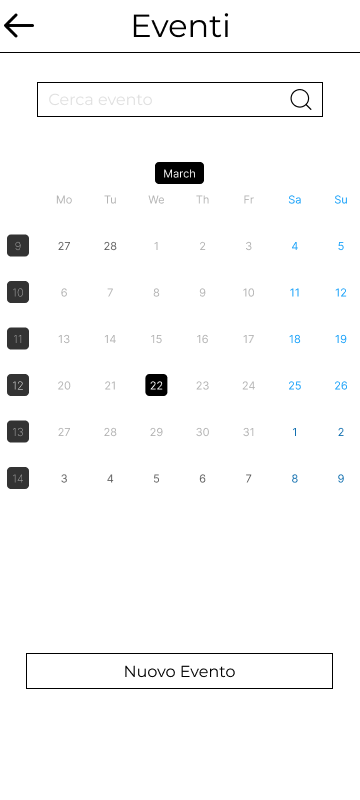
\includegraphics[width=2.4cm]{Eventi.png}}
  \fbox{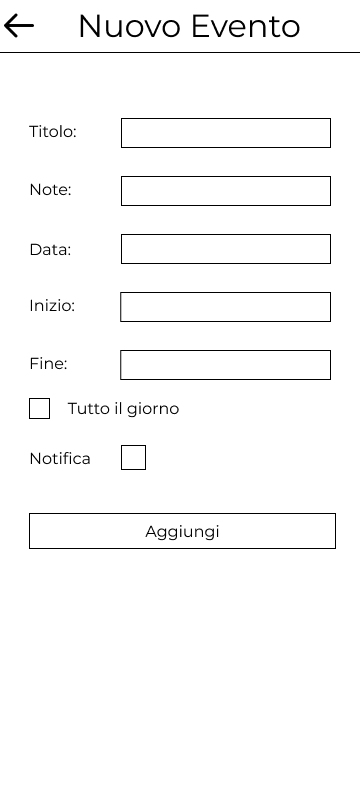
\includegraphics[width=2.4cm]{Aggiungi Evento.png}}
\end{center}

\item \textbf {US6} Come utente autenticato, voglio poter salvare e amministrare le mie carte fedeltà in modo da poter mostrare il codice a barre al negozio cliccando sul nome della tessera. (\hyperlink{RF13}{RF13}, \hyperlink{RF14}{RF14}, \hyperlink{RF15}{RF15}, \hyperlink{RF16}{RF16})

\begin{center}
  \fbox{\includegraphics[width=2.4cm]{Carte Fedeltà.png}}
  \fbox{\includegraphics[width=2.4cm]{Aggiungi Carta Fedeltà.png}}
  \fbox{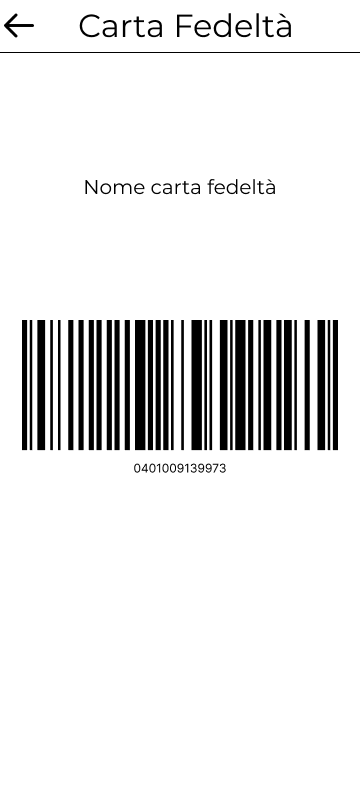
\includegraphics[width=2.4cm]{Esempio Carta.png}}
\end{center}

\item \textbf {US7} Come utente autenticato, voglio poter salvare e gestire i luoghi cui sono stato o che voglio visitare, anche con la propria posizione. Voglio poter categorizzare tutti i luoghi in modo da capire, ad esempio, quali ho già visitato e quali no. (\hyperlink{RF17}{RF17}, \hyperlink{RF18}{RF18}, \hyperlink{RF19}{RF19}, \hyperlink{RF20}{RF20})

\begin{center}
  \fbox{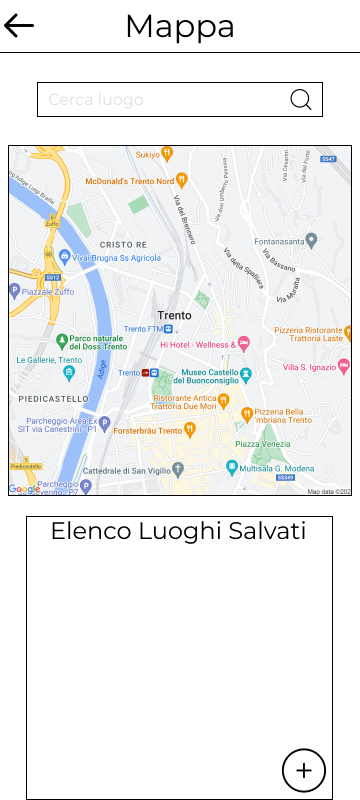
\includegraphics[width=2.4cm]{Mappa.png}}
  \fbox{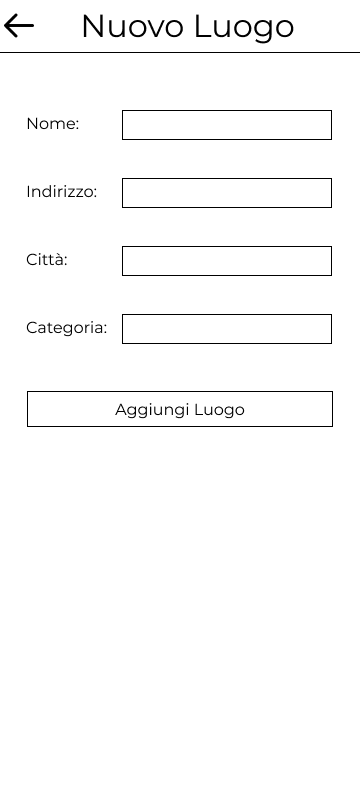
\includegraphics[width=2.4cm]{Aggiungi Luogo.png}}
\end{center}

\item \textbf {US8}  Come utente autenticato, voglio poter salvare e amministrare le mie ricette, inserendo i vari ingredienti e le rispettive quantità e descrivendo i passaggi per la preparazione, in modo da averle sempre a disposizione. Voglio inoltre aggiungere tutti o alcuni degli ingredienti di una specifica ricetta direttamente alla lista della spesa attraverso un bottone, senza dover trascriverli. (\hyperlink{RF21}{RF21}, \hyperlink{RF22}{RF22}, \hyperlink{RF23}{RF23}, \hyperlink{RF24}{RF24})

\begin{center}
  \fbox{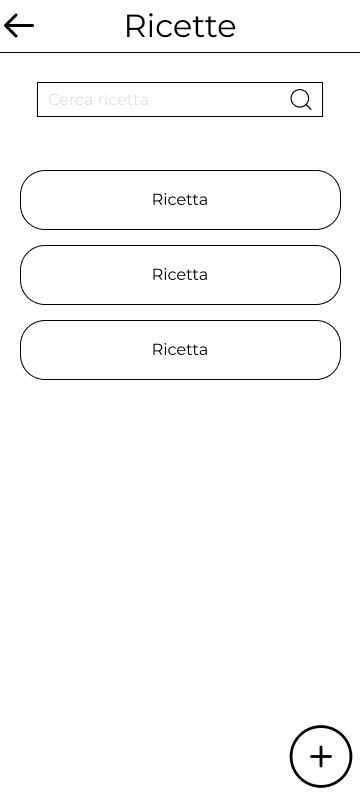
\includegraphics[width=2.4cm]{Ricette.png}}
  \fbox{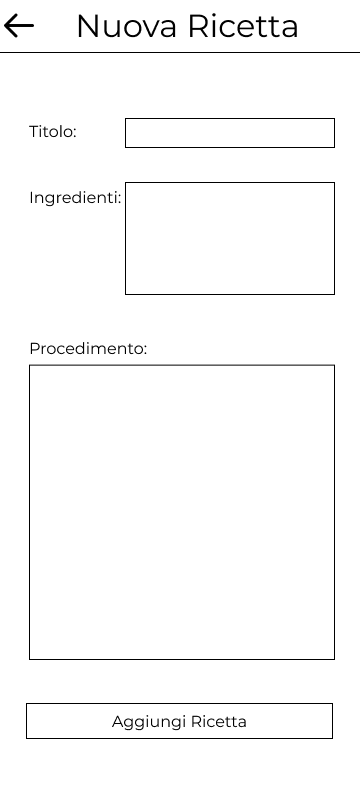
\includegraphics[width=2.4cm]{Nuova Ricetta.png}}
  \fbox{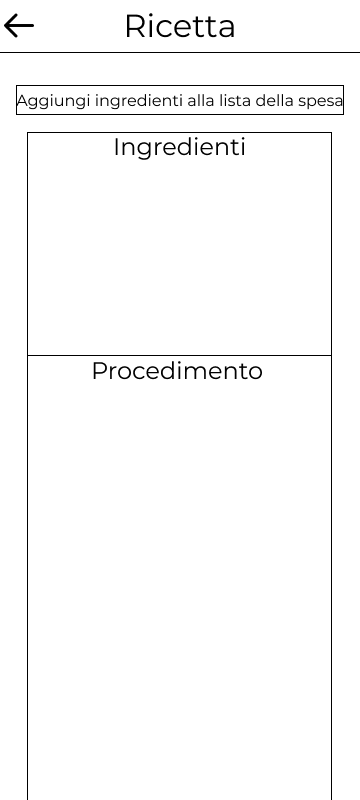
\includegraphics[width=2.4cm]{Esempio Ricetta.png}}
\end{center}

\item \textbf {US9}  Come utente autenticato, voglio poter visualizzare, aggiungere, modificare delle liste, come per esempio la lista della spesa e la to-do List. In ogni lista, voglio poter contrassegnare attraverso una checkbox ogni elemento in modo da evidenziare che di quell'elemento non ho più bisogno. (\hyperlink{RF25}{RF25}, \hyperlink{RF26}{RF26}, \hyperlink{RF27}{RF27}, \hyperlink{RF28}{RF28}, \hyperlink{RF29}{RF29})

\begin{center}
  \fbox{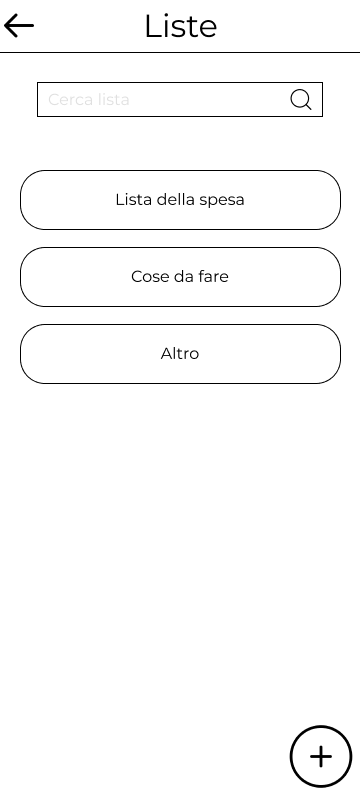
\includegraphics[width=2.4cm]{ListeP.png}}
  \fbox{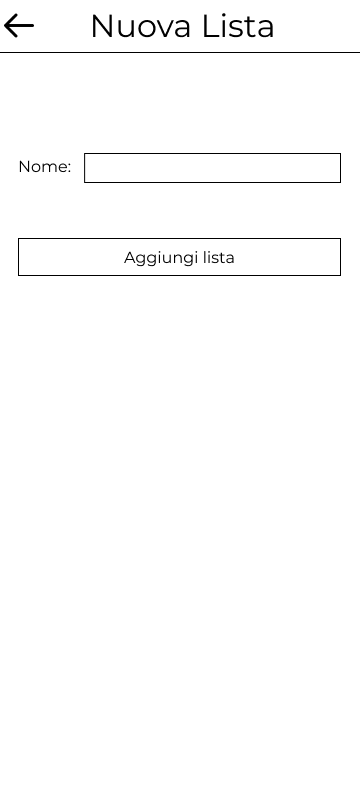
\includegraphics[width=2.4cm]{Aggiungi Lista.png}}
  \fbox{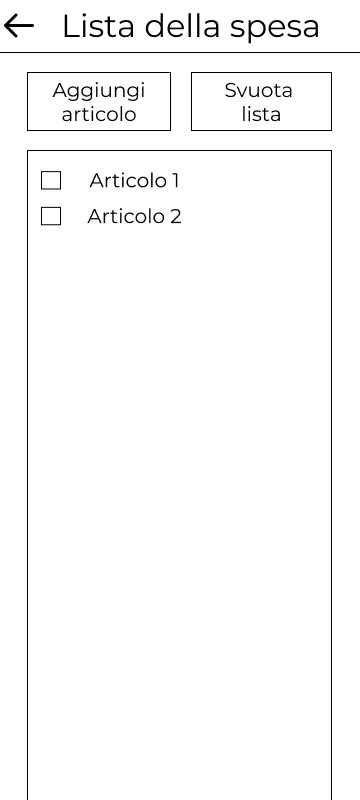
\includegraphics[width=2.4cm]{Lista della spesa.png}}
  \fbox{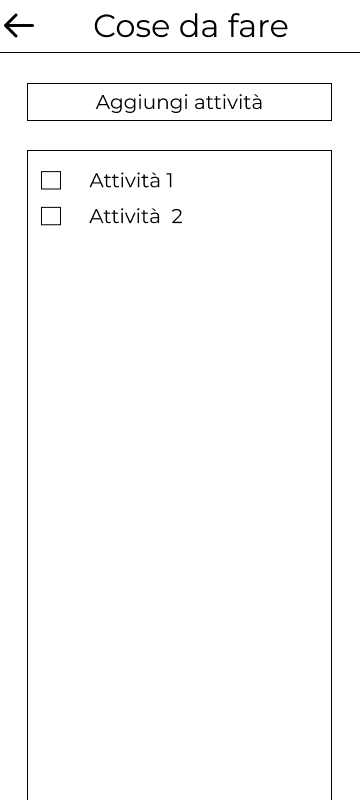
\includegraphics[width=2.4cm]{Cose Da Fare.png}}
  \fbox{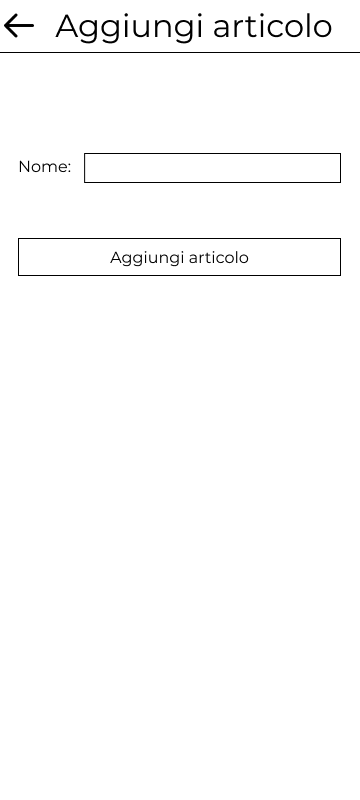
\includegraphics[width=2.4cm]{Aggiungi Articolo.png}}
  \fbox{\includegraphics[width=2.4cm]{Aggiungi Attività.png}}
\end{center}

\end{itemize}

\section*{Requisiti funzionali}
\begin{itemize} \setlength\itemsep{0.01em}
\item \textbf {\hypertarget{RF1}{RF1}} L'applicazione deve permettere a un utente non registrato di registrarsi inserendo in un form: nome, cognome, username, email, password, la quale viene richiesta due volte per evitare errori di inserimento. Una volta completata la registrazione viene inviata una email di benvenuto contenente un link per confermare l'indirizzo email (se l'indirizzo email non viene confermato, l'autenticazione non è ammessa).
\item \textbf {\hypertarget{RF2}{RF2}} L'applicazione deve permettere a un utente registrato di poter accedere al sistema inserendo username o email e password forniti in fase di registrazione.
\item \textbf {\hypertarget{RF3}{RF3}} L'applicazione deve permettere a un utente autenticato la visualizzazione di un menù iniziale dove sono visibili tutte le funzionalità. Le funzionalità presenti sono: gestione budget, liste, eventi, ricette, mappa e carte fedeltà.
\item \textbf {\hypertarget{RF4}{RF4}} L'applicazione deve permettere a un utente autenticato di entrare nella scheda relativa ad ogni funzione quando viene cliccata nel menù iniziale.
\item \textbf {\hypertarget{RF5}{RF5}} L'applicazione deve permettere a un utente autenticato di visualizzare un elenco di movimenti, ordinati dal più recente al meno recente, e di scegliere se visualizzare tutti i movimenti o solamente quelli del mese corrente. L'applicazione deve permettere una visualizzazione grafica del saldo delle varie categorie(\hyperlink{RF7}{RF7}) e un resoconto di entrare e uscite del mese corrente.
\item \textbf {\hypertarget{RF6}{RF6}} L'applicazione deve permettere a un utente autenticato di aggiungere un movimento inserendo l'importo, la tipologia (se è un'entrata o un'uscita) (\hyperlink{RF8}{RF8}), la categoria (\hyperlink{RF7}{RF7}) e delle eventuali note associate. L'applicazione deve consentire di rimuovere o modificare un movimento.
\item \textbf {\hypertarget{RF7}{RF7}} L'applicazione deve permettere a un utente autenticato di associare una categoria ad ogni movimento, di visualizzare tutti i movimenti associati ad ogni categoria, ordinati dal più recente al meno recente, e di scegliere se visualizzare tutti i movimenti o solo quelli del mese corrente.
\item \textbf {\hypertarget{RF8}{RF8}} L'applicazione deve permettere a un utente autenticato di associare una tipologia ad ogni movimento (entrata o uscita), di visualizzare tutti i movimenti associati alla tipologia Entrate e alla tipologia Uscite, ordinati dal più recente al meno recente, e di scegliere se visualizzare tutti i movimenti o solo quelli del mese corrente.
\item \textbf {\hypertarget{RF9}{RF9}} L'applicazione deve permettere a un utente autenticato di cercare uno specifico movimento, secondo il titolo del movimento o le note associate.
\item \textbf {\hypertarget{RF10}{RF10}} L'applicazione deve mostrare a un utente autenticato un calendario, in cui sono mostrati gli eventi nei giorni associati.
\item \textbf {\hypertarget{RF11}{RF11}} L'applicazione deve permettere a un utente autenticato di aggiungere un nuovo evento cliccando sul tasto "aggiungi evento" oppure direttamente sul giorno del calendario in cui desidera aggiungere l'evento, inserendo il titolo, le note, la data, l'ora di inizio e l'ora di fine e se si vuole ricevere una notifica via mail(\hyperlink{RF12}{RF12}). L'applicazione deve consentire l'opzione "tutto il giorno", infatti spuntando la casella l'evento sarà assegnato a tutto il giorno corrispondente, e l'eliminazione o la modifica dell'evento.
\item \textbf {\hypertarget{RF12}{RF12}} L'applicazione, nel caso in cui l'utente autenticato lo desideri, deve inviare una mail all'utente per ricordargli l'evento (l'utente autenticato può scegliere quanto prima riceverla). La mail sarà mandata all'indirizzo email fornito dall'utente in fase di registrazione.
\item \textbf {\hypertarget{RF13}{RF13}} L'applicazione deve mostrare a un utente autenticato un elenco di tutte le carte fedeltà inserite, in cui viene mostrato il nome della carta.
\item \textbf {\hypertarget{RF14}{RF14}} L'applicazione deve mostrare a un utente autenticato, per ogni carta fedeltà, il nome della carta e il codice a barre corrispondente al numero della carta.
\item \textbf {\hypertarget{RF15}{RF15}} L'applicazione deve permettere a un utente autenticato di inserire una nuova carta fedeltà inserendo il nome e il numero della carte. L'applicazione deve creare poi il codice a barre corrispondente al numero fornito.
\item \textbf {\hypertarget{RF16}{RF16}} L'applicazione deve permettere a un utente autenticato di ricercare una specifica carta secondo il nome.
\item \textbf {\hypertarget{RF17}{RF17}} L'applicazione deve mostrare a un utente autenticato una mappa con dei segnalibri sui luoghi salvati dall'utente e un elenco con tutti i luoghi salvati, ordinati dal più recente al meno recente.
\item \textbf {\hypertarget{RF18}{RF18}} L'applicazione deve permettere a un utente autenticato di aggiungere un luogo inserendo il nome, l'indirizzo, la città e può essere assegnato una categoria. L'applicazione deve consentire l'eliminazione o la modifica di un luogo.
\item \textbf {\hypertarget{RF19}{RF19}} L'applicazione deve permettere a un utente autenticato di ricercare uno specifico luogo tramite la barra di ricerca, inserendo il nome.
\item \textbf {\hypertarget{RF20}{RF20}} L'applicazione deve permettere la localizzazione di un utente autenticato tramite GPS e visualizzarne la posizione sulla mappa.
\item \textbf {\hypertarget{RF21}{RF21}} L'applicazione deve mostrare a un utente autenticato una lista delle ricette inserite e, per ogni ricetta, i dettagli di quella ricetta (titolo, ingredienti, procedimento).
\item \textbf {\hypertarget{RF22}{RF22}} L'applicazione deve permettere a un utente autenticato di aggiungere una ricetta inserendo il titolo, gli ingredienti necessari e il procedimento. L'applicazione deve consentire l'eliminazione e la modifica di una ricetta.
\item \textbf {\hypertarget{RF23}{RF23}} L'applicazione deve permettere a un utente autenticato di aggiungere tutti o alcuni degli ingredienti necessari per una ricetta alla lista della spesa.
\item \textbf {\hypertarget{RF24}{RF24}} L'applicazione deve permettere a un utente autenticato di ricercare una specifica ricetta secondo il titolo.
\item \textbf {\hypertarget{RF25}{RF25}} L'applicazione deve mostrare a un utente autenticato le liste salvate e, per ogni lista, visualizzare l'elenco di elementi in tale lista.
\item \textbf {\hypertarget{RF26}{RF26}} L'applicazione deve permettere a un utente autenticato di aggiungere una lista, inserendo il nome, e di modificare o rimuovere una lista.
\item \textbf {\hypertarget{RF27}{RF27}} L'applicazione deve permettere a un utente autenticato di aggiungere e modificare le voci all'interno di una lista. Le voci sono affiancate da una checkbox che può essere spuntata quando non si è più interessati a tale elemento della lista. 
\item \textbf {\hypertarget{RF28}{RF28}} L'applicazione deve permettere di eliminare/svuotare gli elementi della lista contrassegnati.
\item \textbf {\hypertarget{RF29}{RF29}} L'applicazione deve permettere a un utente autenticato di ricercare una specifica lista secondo il nome.
\item \textbf {\hypertarget{RNF30}{RNF30}}  L'applicazione deve permettere a un utente autenticato di entrare nella scheda impostazioni dalla pagina iniziale, dove l'applicazione deve consentire la consultazione dell'informativa sulla privacy, la modifica della lingua dell'applicazione, la visualizzazione delle informazioni sugli sviluppatori e sulla versione attuale e infine la disconnessione. Disconnettendosi l'applicazione reindirizza l'utente nella pagina di login.
\item \textbf {\hypertarget{RNF31}{RNF31}}  L'applicazione deve permettere a un utente autenticato di entrare scheda profilo dalla pagina iniziale, dove l'applicazione deve consentire la visualizzazione della propria foto profilo, il nome e cognome, l'username e la mail e permette la modifica di queste informazioni oltre che della password.
\end{itemize}

\section*{Requisiti non funzionali}
\begin{itemize} \setlength\itemsep{0.01em}

\item \textbf {\hypertarget{RNF1}{RNF1}}  L'applicazione deve supportare l'accesso o la registrazione con Google.
\item \textbf {\hypertarget{RNF2}{RNF2}}  L'applicazione deve permette di recuperare la password se l'utente lo richiede, tramite l'invio di una mail in cui c'è un link per impostare una nuova password.
\item \textbf {\hypertarget{RNF3}{RNF3}}  L'applicazione deve richiedere all'utente se vuole salvare la propria password per ricordare i dati di autenticazione per fare in modo che non debba fare il login ad ogni accesso.
\item \textbf {\hypertarget{RNF4}{RNF4} } L'applicazione deve rispettare il regolamento europeo 2016/679 conosciuto come GDPR, il regolamento generale sulla protezione dei dati.
\item \textbf {\hypertarget{RNF5}{RNF5}} 
La trasmissione dei dati deve avvenire in modo sicuro.
L'applicazione non accetta password troppo deboli.
Le password non sono salvate in chiaro.
\item \textbf {\hypertarget{RNF6}{RNF6}} Un utente deve essere in grado di registrarsi e di imparare ad usare le diverse funzionalità in modo autonomo.
\item \textbf {\hypertarget{RNF7}{RNF7}} L'applicazione deve permettere all'utente di muoversi al suo interno e utilizzarne le funzionalità in modo fluido e senza grossi ritardi o tempi di attesa.

\end{itemize}
%----
\newpage
\section*{Descrizione degli Use case }


\subsection*{1 - Login e registrazione}

\begin{center}
  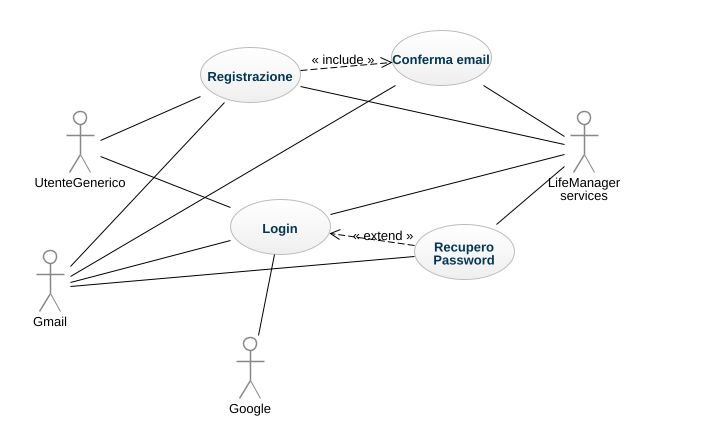
\includegraphics[width=13cm]{UCDloginregistrazione.jpeg}
  \captionof{figure}{Use case login e registrazione}
\end{center}

\subsubsection*{Use case Registrazione}

Questo use case descrive come l'utente non autenticato effettua la registrazione nel sistema tramite form.

\textbf{Descrizione}
\begin{itemize} \setlength\itemsep{0.01em}
\item L'utente non autenticato inserisce nome [nota1], cognome[nota1], username, email[nota2], password[nota3], conferma password[nota3] e preme sul pulsante "Registrati"[nota4] [nota5].
\item Il sistema, tramite Gmail, manda una mail di verifica all'indirizzo specificato, premendo nel link presente nella mail viene effettuata la verifica dell'indirizzo email e visualizzato un messaggio di benvenuto.
\item A registrazione effettuata, si può effettuare il login.
\end{itemize}

\textbf{Note}
\begin{enumerate} \setlength\itemsep{0.01em}
\item Nome e/o cognome non valido (non soddisfano la regex "[a-zA-Z0-9]"), il bordo del campo diventa rosso.
\item Email non valida (non soddisfa la regex ".+@.+..+"), il bordo del campo diventa rosso.
\item Password non valida oppure le due password non sono uguali, il bordo del campo diventa rosso.
\item Ci sono campi non compilati oppure non validi, il bordo di tali campi diventa rosso.
\item L'email inserita è già associata ad un altro account, appare la scritta "Email inserita associata ad un altro account, inserire un'altra email".
\end{enumerate}






\subsubsection*{Use case Login}

Questo use case descrive come l'utente non autenticato effettua il login nel sistema tramite form.

\textbf {Descrizione}
\begin{itemize} \setlength\itemsep{0.01em}
\item L'utente non autenticato, se registrato, inserisce username o email e la sua password e conferma premendo su "Accedi", oppure sceglie l'opzione "Accedi con Google" per accedere tramite il proprio account Google[nota1] [nota2].
\item A login completato, viene visualizzata la HomePage dell'applicazione.
\end{itemize}

\textbf{Note}
\begin{enumerate} \setlength\itemsep{0.01em}
\item Ci sono campi non compilati, il bordo di tali campi diventa rosso.
\item Dati inseriti non corretti, appare la scritta "Utente non presente nel sistema o password inserita errata".
\end{enumerate}

\subsubsection*{Use case conferma email}

Questo use case descrive come avviene la verifica dell'indirizzo email.

\textbf{Descrizione}
\begin{itemize} \setlength\itemsep{0.01em}
\item Il sistema, tramite Gmail, manda una mail di verifica all'indirizzo specificato durante la registrazione, premendo sul link presente nella mail viene effettuata la verifica dell'indirizzo email e visualizzato un messaggio di benvenuto[nota1].
\end{itemize}

\textbf{Note}
\begin{enumerate} \setlength\itemsep{0.01em}
\item Se l'indirizzo email non viene confermato, l'autenticazione non è ammessa.
\end{enumerate}


\subsubsection*{Use case recupero password}

Questo use case descrive come avviene il recupero della password nel caso in cui l'utente autenticato se la sia dimenticata o voglia modificarla.

\textbf{Descrizione}
\begin{itemize} \setlength\itemsep{0.01em}
\item L'utente autenticato clicca sul pulsante "Recupera password".
\item L'utente autenticato inserisce la sua email[nota1] [nota2] e preme su "Invia email di recupero".
\item L'email inviata tramite Gmail permetterà all'utente autenticato di impostare una nuova password.
\end{itemize}

\textbf{Note}
\begin{enumerate} \setlength\itemsep{0.01em}
\item Campo Email non compilato, il bordo del campo diventa rosso.
\item Email inserita non corretta o non associata a nessun account, appare il messaggio "Email inserita non valida".
\end{enumerate}


\subsection*{2 - Home page, impostazioni, profilo}
\begin{center}
  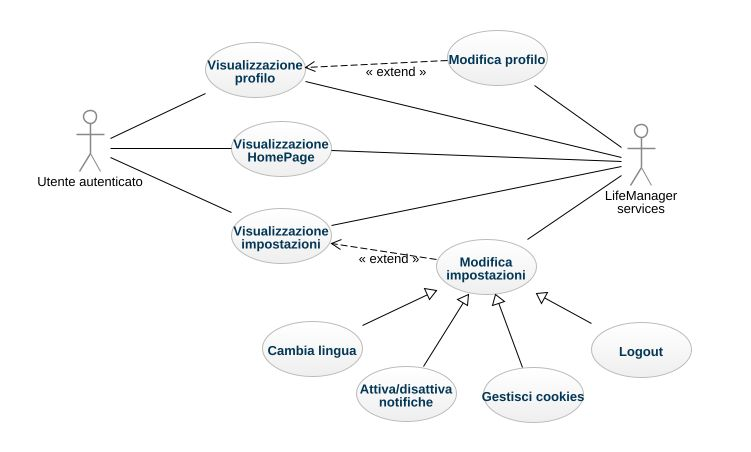
\includegraphics[width=13cm]{UCDHomePage.jpeg}
  \captionof{figure}{Use case Home page, impostazioni, profilo}
\end{center}


\subsubsection*{Use case visualizzazione home page}

Questo use case descrive la visualizzazione della home page da parte di un utente autenticato.

\textbf{Descrizione}
\begin{itemize} \setlength\itemsep{0.01em}
\item L'utente autenticato visualizza la lista delle schede che corrispondono alle varie funzionalità.
\item L'utente può cliccare su ognuna delle schede presenti nella home page.
\end{itemize}


\subsubsection*{Use case visualizzazione profilo}

Questo use case descrive la visualizzazione dei dati associati al proprio profilo da parte di un utente autenticato.

\textbf{Descrizione}
\begin{itemize} \setlength\itemsep{0.01em}
\item L'utente autenticato visualizza le informazioni relative al proprio profilo, come username, email, foto profilo.[nota1]
\end{itemize}

\textbf{Note}
\begin{enumerate} \setlength\itemsep{0.01em}
\item L'utente non è tenuto a specificare una foto profilo, può lasciare l'icona generica (vuota).
\end{enumerate}

\subsubsection*{Use case modifica profilo}

Questo use case descrive come l'utente possa andare a modificare le informazioni associate al proprio profilo.

\textbf{Descrizione}
\begin{itemize} \setlength\itemsep{0.01em}
\item L'utente autenticato modifica la foto profilo premendo sull'icona della matita e scegliendo un'immagine a suo piacimento.
\item L'utente autenticato modifica nome e cognome premendo sull'icona della matita[nota3].
\item L'utente autenticato preme il pulsante "Modifica profilo" se ha necessità di cambiare username, email [nota1], password [nota2] [nota3] [nota4].
\end{itemize}

\textbf{Note}
\begin{enumerate} \setlength\itemsep{0.01em}
\item Email non valida (non soddisfa la regex ".+@.+..+"), il bordo del campo diventa rosso.
\item Password non valida oppure le due password non sono uguali, il bordo del campo diventa rosso.
\item Ci sono campi non compilati oppure non validi, il bordo di tali campi diventa rosso.
\item L'email inserita è già associata ad un altro account, appare la scritta "Email inserita associata ad un altro account, inserire un'altra email".
\end{enumerate}

\subsubsection*{Use case visualizzazione impostazioni}

Questo use case descrive la visualizzazione delle impostazioni del sistema da parte di un utente autenticato.

\textbf{Descrizione}
\begin{itemize} \setlength\itemsep{0.01em}
\item L'utente autenticato visualizza se le notifiche sono attivate o meno premendo sul pulsante "Notifiche".
\item L'utente autenticato visualizza le informazioni relative a privacy e sicurezza, in particolare l'informativa sul trattamento dei dati personali e la gestione dei cookies, premendo su "Privacy e sicurezza" .
\item L'utente autenticato visualizza la lingua impostata per il sistema premendo il pulsante "Lingua".
\item L'utente autenticato visualizza le informazioni generali del sistema, come la versione attuale dell'applicazione e i contatti degli sviluppatori.
\end{itemize}

\subsubsection*{Use case gestione impostazioni}

Questo use case descrive come l'utente autenticato effettua modifiche alle impostazioni del sistema premendo sul bottone relativo alla funzionalità/impostazione che vuole modificare.


\subsubsection*{Use case cambia lingua}

Questo use case descrive come l'utente autenticato modifica la lingua del sistema, scegliendo tra una lista di lingue predefinite.

\textbf{Descrizione}
\begin{itemize} \setlength\itemsep{0.01em}
\item L'utente autenticato cambia la lingua cliccando sull' apposito bottone e scegliendo tra una serie di lingue da un menù a tendina.
\end{itemize}

\subsubsection*{Use case gestione cookies}

Questo use case descrive come l'utente autenticato modifica le proprie preferenze riguardanti i cookies.

\textbf{Descrizione}
\begin{itemize} \setlength\itemsep{0.01em}
\item L'utente autenticato cambia le impostazioni dei cookies cliccando sull'apposito bottone, scegliendo se accettarli, accettare solo quelli essenziali o rifiutarli.
\end{itemize}

\subsubsection*{Use case logout}

Questo use case descrive come l'utente autenticato effettua il logout.

\textbf{Descrizione}
\begin{itemize} \setlength\itemsep{0.01em}
\item L'utente autenticato si disconnette in modo sicuro attraverso l'apposito bottone [nota1].
\end{itemize}

\textbf{Note}
\begin{enumerate} \setlength\itemsep{0.01em}
\item Il sistema visualizza un banner per permettere all'utente di confermare il logout.
\end{enumerate}


\subsection*{3 - Budget}

\begin{center}
  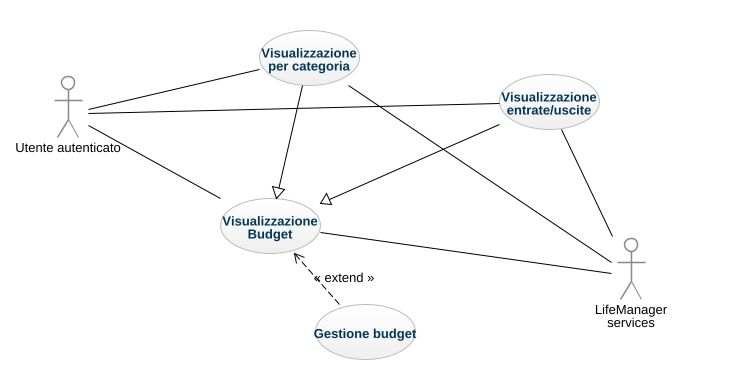
\includegraphics[width=13cm]{UCDbudget.jpeg}
  \captionof{figure}{Use case Budget}
\end{center}

\subsubsection*{Use case visualizzazione budget}

Questo use case descrive la visualizzazione da parte dell'utente autenticato del proprio budget e le informazioni relative ai propri movimenti.

\textbf{Descrizione}
\begin{itemize} \setlength\itemsep{0.01em}
\item L'utente autenticato visualizza una presentazione grafica delle categorie in cui ogni movimento è classificato, relativa al mese corrente.
\item L'utente autenticato visualizza il riepilogo delle entrate e delle uscite del mese corrente.
\item L'utente autenticato visualizza l'elenco di tutti i suoi movimenti ordinati in base a quando sono stati inseriti[nota1] e con la possibilità di essere filtrati [nota2]
\item L'utente autenticato può cercare un determinato movimento premendo il pulsante "Cerca" [nota3].
\end{itemize}

\textbf{Note}
\begin{enumerate} \setlength\itemsep{0.01em}
\item Dal più recente a quello meno recente.
\item E' possibile filtrare i movimenti secondo il mese corrente.
\item La ricerca viene effettuata in base al nome del movimento o delle note associate a esso.
\end{enumerate}


\subsubsection*{Use case visualizzazione per categoria}

Questo use case descrive la visualizzazione da parte dell'utente autenticato del proprio budget relativo a una determinata categoria e le informazioni sui movimenti associati a tale categoria.

\textbf{Descrizione}
\begin{itemize} \setlength\itemsep{0.01em}
\item L'utente autenticato, cliccando sulla categoria che desidera ispezionare, visualizza l'elenco dei movimenti associati a tale categoria [nota1] e con la possibilità di essere filtrati [nota2].
\item L'utente autenticato può cercare un determinato movimento nella lista di movimenti della categoria desiderata con il pulsante "Cerca" [nota3].
\end{itemize}

\textbf{Note}
\begin{enumerate} \setlength\itemsep{0.01em}
\item Dal più recente a quello meno recente.
\item E' possibile filtrare i movimenti secondo il mese corrente.
\item La ricerca viene effettuata in base al nome del movimento o delle note associate a esso.
\end{enumerate}



\subsubsection*{Use case visualizzazione entrate/uscite}

Questo use case descrive la visualizzazione da parte dell'utente autenticato delle proprie entrate o delle proprie uscite.

\textbf{Descrizione}
\begin{itemize} \setlength\itemsep{0.01em}
\item L'utente autenticato, cliccando su "Entrate" o su "Uscite", visualizza rispettivamente l'elenco dei movimenti in entrata o l'elenco dei movimenti in uscita [nota1] e con la possibilità di essere filtrati [nota2].
\item L'utente autenticato può cercare un determinato movimento nella lista di movimenti in entrata/uscita con il pulsante "Cerca" [nota3].
\end{itemize}

\textbf{Note}
\begin{enumerate} \setlength\itemsep{0.01em}
\item Dal più recente a quello meno recente.
\item E' possibile filtrare i movimenti secondo il mese corrente.
\item La ricerca viene effettuata in base al nome del movimento o delle note associate a esso.
\end{enumerate}




\subsubsection*{Use case gestione budget}

Questo use case descrive come l'utente autenticato può aggiungere, rimuovere o modificare movimenti e aggiungere, rimuovere o modificare le categorie in cui i movimenti sono classificate.


\subsubsection*{Use case aggiungi categoria}

Questo use case descrive come l'utente autenticato inserisce una nuova categoria di movimenti.

\textbf{Descrizione}
\begin{itemize} \setlength\itemsep{0.01em}
\item L'utente autenticato aggiunge una categoria con il bottone "+" presente nel grafico delle categorie [nota1] [nota2].
\end{itemize}

\textbf{Note}
\begin{enumerate} \setlength\itemsep{0.01em}
\item Nell'aggiunta di una categoria, l'utente autenticato inserisce obbligatoriamente il nome di tale categoria.
\item Il campo nome non può essere vuoto, se accade i bordi del campo diventano rossi.
\end{enumerate}




\subsubsection*{Use case modifica categoria}

Questo use case descrive come l'utente autenticato modifica una categoria esistente di movimenti.

\textbf{Descrizione}
\begin{itemize} \setlength\itemsep{0.01em}
\item L'utente autenticato modifica una categoria tenendo premuta tale categoria nel grafico delle categorie e scegliendo l'opzione "Modifica" nel menu che appare [nota1] [nota2].
\end{itemize}

\textbf{Note}
\begin{enumerate} \setlength\itemsep{0.01em}
\item Nella modifica di una categoria, l'utente autenticato modifica il nome di tale categoria.
\item Il campo nome non può essere vuoto, se accade i bordi del campo diventano rossi.
\end{enumerate}



\subsubsection*{Use case elimina categoria}

Questo use case descrive come l'utente autenticato elimina una categoria esistente di movimenti.

\textbf{Descrizione}
\begin{itemize} \setlength\itemsep{0.01em}
\item L'utente autenticato elimina una categoria tenendo premuta tale categoria nel grafico delle categorie e scegliendo l'opzione "Elimina" nel menu che appare [nota1].
\end{itemize}

\textbf{Note}
\begin{enumerate} \setlength\itemsep{0.01em}
\item Il sistema visualizzerà un banner chiedendo all'utente di confermare l'eliminazione  (vedi use case Conferma eliminazione).
\end{enumerate}



\subsubsection*{Use case aggiungi movimento}

Questo use case descrive come l'utente autenticato aggiunge un nuovo movimento .

\textbf{Descrizione}
\begin{itemize} \setlength\itemsep{0.01em}
\item L'utente autenticato aggiunge un nuovo movimento premendo il pulsante "+" presente nell'elenco dei movimenti, oppure presente nella categoria selezionata o nella sezione "Entrate"/"Uscite" selezionata [nota1] [nota2] [nota3] [nota4].
\end{itemize}

\textbf{Note}
\begin{enumerate} \setlength\itemsep{0.01em}
\item Nell'aggiunta di un movimento, l'utente autenticato inserisce obbligatoriamente titolo, importo, tipologia (entrata o uscita), categoria (tra le categorie presenti) e opzionalmente eventuali note.
\item Se l'aggiunta di un movimento avviene da una scheda relativa ad una categoria specifica, il campo categoria sarà pre-impostato secondo la tale categoria.
\item Se l'aggiunta di un movimento avviene dalla scheda "Entrate" o dalla scheda "Uscite", il campo tipologia sarà pre-impostato secondo la tale scheda.
\item I campi titolo, importo, tipologia e categoria non possono essere vuoti, se accade i bordi del campo diventano rossi.
\end{enumerate}


\subsubsection*{Use case modifica movimento}

Questo use case descrive come l'utente autenticato modifica un movimento esistente.

\textbf{Descrizione}
\begin{itemize} \setlength\itemsep{0.01em}
\item L'utente autenticato modifica un movimento esistente tenendo premuto tale movimento e selezionando l'opzione "Modifica" nel menù che appare [nota1] [nota2].
\end{itemize}

\textbf{Note}
\begin{enumerate} \setlength\itemsep{0.01em}
\item Nella modifica di un movimento, l'utente autenticato modifica uno o più campi relativi a tale movimento (titolo, importo, tipologia, categoria, note) .
\item I campi titolo, importo, tipologia e categoria non possono essere vuoti, se accade i bordi del campo diventano rossi.
\end{enumerate}



\subsubsection*{Use case elimina movimento}

Questo use case descrive come l'utente autenticato elimina un movimento esistente.

\textbf{Descrizione}
\begin{itemize} \setlength\itemsep{0.01em}
\item L'utente autenticato elimina un movimento tenendo premuto tale movimento e scegliendo l'opzione "Elimina" nel menu che appare [nota1].
\end{itemize}

\textbf{Note}
\begin{enumerate} \setlength\itemsep{0.01em}
\item Il sistema visualizzerà un banner chiedendo all'utente di confermare l'eliminazione  (vedi use case Conferma eliminazione).
\end{enumerate}



\subsection*{4 - Liste di interesse}

\begin{center}
  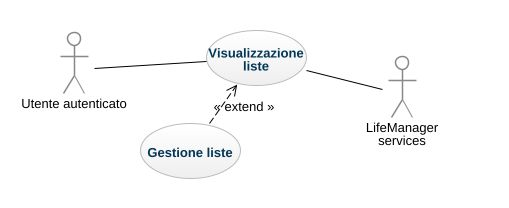
\includegraphics[width=13cm]{UCDliste.jpeg}
  \captionof{figure}{Use case liste di interesse}
\end{center}
\subsubsection*{Use case visualizzazione liste}

Questo use case descrive la visualizzazione da parte dell'utente autenticato dell'elenco delle proprie liste di interesse [nota1].

\textbf{Descrizione}
\begin{itemize} \setlength\itemsep{0.01em}
\item L'utente autenticato visualizza l'elenco delle proprie liste.
\item L'utente autenticato può cercare una determinata lista con il pulsante "Cerca" [nota2].
\end{itemize}

\textbf{Note}
\begin{enumerate} \setlength\itemsep{0.01em}
\item Le liste predefinite sono: lista della spesa, to-do List e altro.
\item La ricerca avviene secondo il nome della lista.
\end{enumerate}




\subsubsection*{Use case visualizzazione elementi lista}

Questo use case descrive la visualizzazione da parte dell'utente autenticato degli elementi appartenenti ad una specifica lista.

\textbf{Descrizione}
\begin{itemize} \setlength\itemsep{0.01em}
\item L'utente autenticato visualizza l'elenco di elementi appartenenti a tale lista, compresi quelli a cui non è più interessato[nota1].
\end{itemize}

\textbf{Note}
\begin{enumerate} \setlength\itemsep{0.01em}
\item Gli elementi a cui non è più interessato sono contrassegnati con un box e appaiono sbarrati e sbiaditi.
\end{enumerate}



\subsubsection*{Use case gestione liste}

Questo use case descrive come l'utente autenticato può aggiungere, rimuovere o modificare l'elenco delle proprie liste di interesse.


\subsubsection*{Use case aggiungi lista}

Questo use case descrive l'aggiunta da parte dell'utente autenticato di una nuova lista di interesse.

\textbf{Descrizione}
\begin{itemize} \setlength\itemsep{0.01em}
\item L'utente autenticato aggiunge una lista con il bottone "+" presente nella scheda Liste [nota1] [nota2].
\end{itemize}

\textbf{Note}
\begin{enumerate} \setlength\itemsep{0.01em}
\item Nell'aggiunta di una lista, l'utente autenticato inserisce obbligatoriamente il nome di tale lista.
\item Il campo nome non può essere vuoto, se accade i bordi del campo diventano rossi.
\end{enumerate}


\subsubsection*{Use case modifica lista}

Questo use case descrive la modifica da parte dell'utente autenticato di una lista di interesse esistente.

\textbf{Descrizione}
\begin{itemize} \setlength\itemsep{0.01em}
\item L'utente autenticato modifica una lista tenendo premuta tale lista e scegliendo l'opzione "Modifica" nel menu che appare [nota1][nota2].
\end{itemize}

\textbf{Note}
\begin{enumerate} \setlength\itemsep{0.01em}
\item Nella modifica di una lista, l'utente autenticato modifica il nome di tale lista.
\item Il campo nome non può essere vuoto, se accade i bordi del campo diventano rossi.
\end{enumerate}



\subsubsection*{Use case elimina lista}

Questo use case descrive come l'utente autenticato elimina una lista di interesse esistente.

\textbf{Descrizione}
\begin{itemize} \setlength\itemsep{0.01em}
\item L'utente autenticato elimina una lista tenendo premuta tale lista e scegliendo l'opzione "Elimina" nel menu che appare [nota1].
\end{itemize}

\textbf{Note}
\begin{enumerate} \setlength\itemsep{0.01em}
\item Il sistema visualizzerà un banner chiedendo all'utente di confermare l'eliminazione (vedi use case Conferma eliminazione).
\end{enumerate}





\subsubsection*{Use case gestione elementi nella lista}

Questo use case descrive come l'utente autenticato gestisce gli elementi di una specifica lista, in particolare per ogni lista può aggiungere, rimuovere o modificare gli elementi.


\subsubsection*{Use case aggiungi elemento nella lista}

Questo use case descrive l'aggiunta da parte dell'utente autenticato di elementi in una lista di interesse specifica.

\textbf{Descrizione}
\begin{itemize} \setlength\itemsep{0.01em}
\item Per ogni lista, l'utente autenticato aggiunge uno o più elementi alla lista con il bottone "Aggiungi" [nota1] [nota2].
\end{itemize}

\textbf{Note}
\begin{enumerate} \setlength\itemsep{0.01em}
\item Nell'aggiunta di un elemento alla lista, l'utente autenticato inserisce obbligatoriamente il nome di tale elemento.
\item Il campo nome non può essere vuoto, se accade i bordi del campo diventano rossi.
\end{enumerate}



\subsubsection*{Use case modifica singolo elemento}

Questo use case descrive la modifica da parte dell'utente autenticato di un elemento esistente nella lista di interesse.

\textbf{Descrizione}
\begin{itemize} \setlength\itemsep{0.01em}
\item L'utente autenticato modifica un elemento nella lista tenendo premuto tale elemento e scegliendo l'opzione "Modifica" nel menu che appare [nota1][nota2].
\end{itemize}

\textbf{Note}
\begin{enumerate} \setlength\itemsep{0.01em}
\item Nella modifica di un elemento nella lista, l'utente autenticato modifica il nome di tale elemento (nome elemento).
\item Il campo nome non può essere vuoto, se accade i bordi del campo diventano rossi.
\end{enumerate}




\subsubsection*{Use case contrassegna elemento}

Questo use case descrive come l'utente contrassegna un elemento di una lista di interesse.

\textbf{Descrizione}
\begin{itemize} \setlength\itemsep{0.01em}
\item L'utente autenticato contrassegna gli elementi della lista una volta che non ne ha più bisogno; per farlo, clicca sul box in fianco all'elemento che vuole contrassegnare[nota1].
\end{itemize}

\textbf{Note}
\begin{enumerate} \setlength\itemsep{0.01em}
\item Gli elementi contrassegnati verranno barrati e sbiaditi nell'elenco degli elementi.
\end{enumerate}



\subsubsection*{Use case svuota lista}

Questo use case descrive come l'utente svuota una lista degli elementi di cui non è più interessato.

\textbf{Descrizione}
\begin{itemize} \setlength\itemsep{0.01em}
\item L'utente autenticato svuota la lista quando non è più interessato agli elementi in tale lista, in particolare elimina dalla lista gli elementi contrassegnati.
\end{itemize}

\textbf{Note}
\begin{enumerate} \setlength\itemsep{0.01em}
\item Il sistema visualizzerà un banner chiedendo all'utente di confermare lo svuotamento della lista.
\end{enumerate}







\subsection*{4 - Eventi }

\begin{center}
  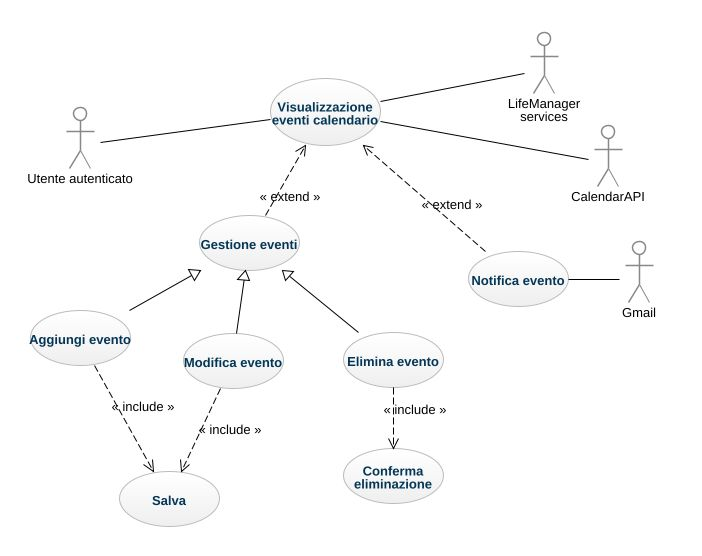
\includegraphics[width=13cm]{UCDeventi.jpeg}
  \captionof{figure}{Use case eventi}
\end{center}
\subsubsection*{Use case visualizzazione eventi e calendario}

Questo use case descrive la visualizzazione da parte dell'utente autenticato dei propri eventi o impegni in un calendario [nota1] e la visualizzazione dei dettagli di ogni evento se cliccato.

\textbf{Descrizione}
\begin{itemize} \setlength\itemsep{0.01em}
\item L'utente autenticato visualizza il calendario con segnalati i propri eventi.
\item Per ogni evento, l'utente autenticato visualizza i dettagli relativi a tale evento [nota2].
\end{itemize}

\textbf{Note}
\begin{enumerate} \setlength\itemsep{0.01em}
\item Calendario fornito da Google.
\item I dettagli comprendono titolo, note, giorno, orari di inizio e fine (o tutto il giorno) in cui accade.
\end{enumerate}

\subsubsection*{Use case gestione eventi}

Questo use case descrive come l'utente autenticato può aggiungere, rimuovere o modificare eventi nel calendario.




\subsubsection*{Use case aggiungi evento}

Questo use case descrive come l'utente autenticato può aggiungere un nuovo evento nel calendario.


\textbf{Descrizione}
\begin{itemize} \setlength\itemsep{0.01em}
\item L'utente autenticato aggiunge un nuovo evento cliccando su un giorno del calendario[nota1] oppure con il bottone "Aggiungi evento" [nota2] [nota3].
\end{itemize}

\textbf{Note}
\begin{enumerate} \setlength\itemsep{0.01em}
\item La data del giorno selezionato sarà pre-impostata nella scheda di aggiunta di un evento.
\item Nell'aggiunta di un evento, l'utente autenticato inserisce obbligatoriamente titolo, la data, ora di inizio e fine (o se tutto il giorno contrassegna il box "Tutto il giorno") e opzionalmente inserisce delle note relative a quell'evento.
\item I campi relativi a titolo data e ora di inizio e fine (o tutto il giorno) non possono essere vuoti, se accade il bordo di tali campi diventa rosso.
\end{enumerate}



\subsubsection*{Use case modifica evento}

Questo use case descrive come l'utente autenticato può modificare eventi nel calendario.


\textbf{Descrizione}
\begin{itemize} \setlength\itemsep{0.01em}
\item L'utente autenticato modifica un evento esistente tenendo premuto tale evento nella lista e selezionando "Modifica"  [nota1] [nota2].
\end{itemize}

\textbf{Note}
\begin{enumerate} \setlength\itemsep{0.01em}
\item Nella modifica di un evento, l'utente autenticato modifica uno o più campi relativi all'evento (titolo, data, ora di inizio/fine o tutto il giorno) .
\item I campi relativi a titolo data e ora di inizio e fine (o tutto il giorno) non possono essere vuoti, se accade il bordo di tali campi diventa rosso.
\end{enumerate}




\subsubsection*{Use case elimina evento}

Questo use case descrive come l'utente autenticato può eliminare eventi nel calendario.


\textbf{Descrizione}
\begin{itemize} \setlength\itemsep{0.01em}
\item L'utente autenticato elimina un evento esistente tenendo premuto tale evento nella lista e selezionando "Elimina"  [nota1].
\end{itemize}

\textbf{Note}
\begin{enumerate} \setlength\itemsep{0.01em}
\item Il sistema visualizzerà un banner chiedendo all'utente di confermare l'eliminazione dell'evento  (vedi use case Conferma eliminazione).
\end{enumerate}




\subsubsection*{Use case notifica evento}

Questo use case descrive come l'utente autenticato attiva la notifica di un evento.

\textbf{Descrizione}
\begin{itemize} \setlength\itemsep{0.01em}
\item L'utente autenticato, se desidera ricevere una notifica per ricordargli di un determinato evento, contrassegna il box "Notifica"[nota1].
\end{itemize}

\textbf{Note}
\begin{enumerate} \setlength\itemsep{0.01em}
\item Se contrassegnato il box, l'utente autenticato potrà anche scegliere quanto prima vuole ricevere la notifica.
\end{enumerate}







\subsection*{5 - Ricette }

\begin{center}
  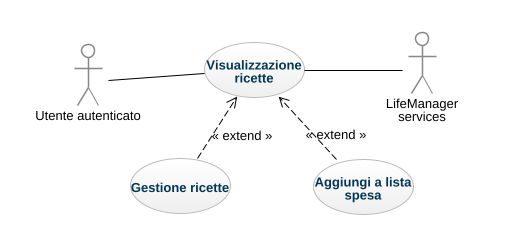
\includegraphics[width=13cm]{UCDricette.jpeg}
  \captionof{figure}{Use case ricette}
\end{center}

\subsubsection*{Use case visualizzazione elenco ricette}

Questo use case descrive la visualizzazione da parte dell'utente autenticato della propria lista di ricette.

\textbf{Descrizione}
\begin{itemize} \setlength\itemsep{0.01em}
\item L'utente autenticato visualizza un elenco con le proprie ricette.
\item L'utente autenticato può cercare una determinata ricetta con il pulsante "Cerca" [nota1].
\end{itemize}

\textbf{Note}
\begin{enumerate} \setlength\itemsep{0.01em}
\item La ricerca avviene secondo il titolo della ricetta.
\end{enumerate}



\subsubsection*{Use case visualizzazione singola ricetta}

Questo use case descrive  la visualizzazione dettagliata da parte dell'utente autenticato di una singola ricetta se cliccata.

\textbf{Descrizione}
\begin{itemize} \setlength\itemsep{0.01em}
\item L'utente autenticato visualizza i dettagli di tale ricetta [nota1].
\end{itemize}

\textbf{Note}
\begin{enumerate} \setlength\itemsep{0.01em}
\item I dettagli della ricetta comprendono titolo, ingredienti, procedimento.
\end{enumerate}







\subsubsection*{Use case gestione ricette}

Questo use case descrive come l'utente autenticato può aggiungere, rimuovere o modificare le proprie ricette.




\subsubsection*{Use case aggiungi ricetta}

Questo use case descrive come l'utente autenticato può aggiungere una nuova ricetta.

\textbf{Descrizione}
\begin{itemize} \setlength\itemsep{0.01em}
\item L'utente autenticato aggiunge una ricetta con il bottone "+" presente nella scheda Ricette [nota1] [nota2].
\end{itemize}

\textbf{Note}
\begin{enumerate} \setlength\itemsep{0.01em}
\item Nell'aggiunta di una nuova ricetta, l'utente autenticato inserisce obbligatoriamente un titolo e uno o più ingredienti e opzionalmente la descrizione del procedimento.
\item I campi relativi a titolo e ingredienti non possono essere vuoti, se accade il bordo di tali campi diventa rosso.
\end{enumerate}



\subsubsection*{Use case modifica ricetta}

Questo use case descrive come l'utente autenticato può modificare una ricetta esistente.

\textbf{Descrizione}
\begin{itemize} \setlength\itemsep{0.01em}
\item L'utente autenticato modifica una ricetta esistente tenendo premuta tale ricetta nella lista e selezionando "Modifica" [nota1] [nota2].
\end{itemize}

\textbf{Note}
\begin{enumerate} \setlength\itemsep{0.01em}
\item Nella modifica di una ricetta, l'utente autenticato modifica uno o più campi riguardanti la ricetta (titolo, ingredienti, procedimento).
\item I campi relativi a titolo e ingredienti non possono essere vuoti, se accade il bordo di tali campi diventa rosso.
\end{enumerate}



\subsubsection*{Use case elimina ricetta}

Questo use case descrive come l'utente autenticato può rimuovere le proprie ricette.

\textbf{Descrizione}
\begin{itemize} \setlength\itemsep{0.01em}
\item L'utente autenticato rimuove una ricetta esistente tenendo premuta tale ricetta nella lista e selezionando "Rimuovi" tra le opzioni che appaiono [nota1].
\end{itemize}

\textbf{Note}
\begin{enumerate} \setlength\itemsep{0.01em}
\item Il sistema visualizzerà un banner chiedendo all'utente di confermare l'eliminazione della ricetta  (vedi use case Conferma eliminazione).
\end{enumerate}




\subsubsection*{Use case aggiunta alla lista della spesa}

 Questo use case descrive l'aggiunta da parte dell'utente autenticato di ingredienti della ricetta direttamente alla lista della spesa.
 
\textbf{Descrizione}
\begin{itemize} \setlength\itemsep{0.01em}
\item L'utente autenticato può aggiungere tutti gli ingredienti di una ricetta alla lista della spesa con il pulsante "Aggiungi a lista della spesa".
\item Per ogni ricetta, l'utente autenticato può aggiungere gli ingredienti che desidera alla lista della spesa tenendo premuti tali ingredienti e selezionando "Aggiungi a lista della spesa".
\end{itemize}







\subsection*{6 - Mappa e luoghi di interesse }

\begin{center}
  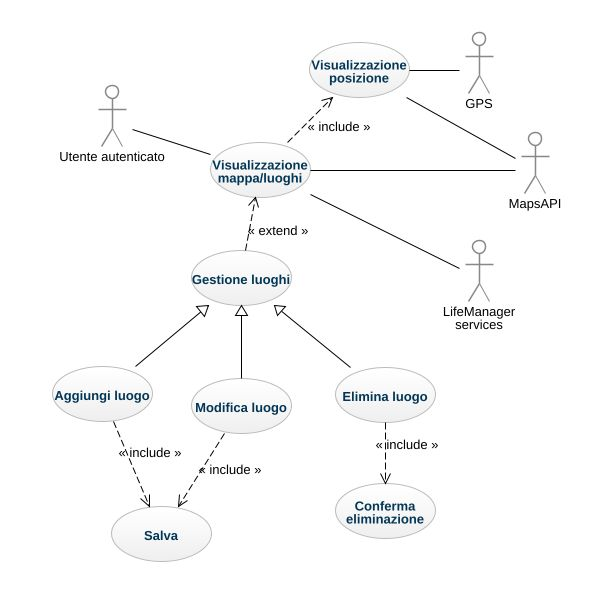
\includegraphics[width=13cm]{UCDluoghi.jpeg}
  \captionof{figure}{Use case Mappa e luoghi di interesse}
\end{center}



\subsubsection*{Use case visualizzazione mappa/luoghi}

Questo use case descrive la visualizzazione da parte dell'utente autenticato della mappa contenente dei riferimenti a luoghi di interesse e la lista di questi luoghi.

\textbf{Descrizione}
\begin{itemize} \setlength\itemsep{0.01em}
\item L'utente autenticato visualizza la mappa con segnalati i propri luoghi di interesse[nota1].
\item L'utente autenticato visualizza l'elenco dei propri luoghi di interesse[nota2].
\item L'utente autenticato può cercare un determinato luogo di interesse con il pulsante "Cerca" [nota3].
\end{itemize}

\textbf{Note}
\begin{enumerate} \setlength\itemsep{0.01em}
\item La mappa è fornita da OpenStreetMap.
\item L'elenco è ordinato cronologicamente in base a quando è stato inserito il luogo di interesse.
\item La ricerca avviene secondo il nome associato al luogo di interesse.
\end{enumerate}




\subsubsection*{Use case gestione luoghi di interesse}

Questo use case descrive come l'utente autenticato può aggiungere, rimuovere o modificare i propri luoghi di interesse.



\subsubsection*{Use case aggiungi luogo}

Questo use case descrive come l'utente autenticato può aggiungere un nuovo luogo di interesse.

\textbf{Descrizione}
\begin{itemize} \setlength\itemsep{0.01em}
\item L'utente autenticato aggiunge un nuovo luogo di interesse con il bottone "+" presente nella scheda Ricette [nota1] [nota3] [nota4].
\item Opzionalmente, l'utente autenticato aggiunge un nuovo luogo di interesse cliccandolo direttamente sulla mappa [nota2].
\end{itemize}

\textbf{Note}
\begin{enumerate} \setlength\itemsep{0.01em}
\item Nell'aggiunta di un nuovo luogo di interesse, l'utente autenticato inserisce obbligatoriamente un nome, un indirizzo e la città, e opzionalmente la categoria relativa al luogo.
\item I campi relativi al luogo selezionato verranno, se possibile, auto-compilati.
\item I campi relativi a nome e indirizzo non possono essere vuoti, se accade il bordo di tali campi diventa rosso.
\item Nel caso in cui l'indirizzo inserito non sia corretto o valido, il bordo del campo si colora di rosso.
\end{enumerate}



\subsubsection*{Use case modifica luogo}

Questo use case descrive come l'utente autenticato può modificare i propri luoghi di interesse esistenti.

\textbf{Descrizione}
\begin{itemize} \setlength\itemsep{0.01em}
\item L'utente autenticato modifica un luogo di interesse esistente tenendo premuto tale luogo nell'elenco e selezionando "Modifica" tra le opzioni che appaiono [nota1] [nota2] [nota3].
\end{itemize}

\textbf{Note}
\begin{enumerate} \setlength\itemsep{0.01em}
\item Nella modifica di un luogo di interesse, l'utente autenticato modifica uno o più campi riguardanti tale luogo (nome, indirizzo, città, categoria).
\item I campi relativi a nome e indirizzo non possono essere vuoti, se accade il bordo di tali campi diventa rosso.
\item Nel caso in cui l'indirizzo inserito non sia corretto o valido, il bordo del campo si colora di rosso.
\end{enumerate}




\subsubsection*{Use case elimina luogo}

Questo use case descrive come l'utente autenticato può  rimuovere  i propri luoghi di interesse esistenti.

\textbf{Descrizione}
\begin{itemize} \setlength\itemsep{0.01em}
\item L'utente autenticato rimuove un luogo di interesse esistente tenendo premuto tale luogo nell'elenco e selezionando "Rimuovi" tra le opzioni che appaiono [nota1].
\end{itemize}

\textbf{Note}
\begin{enumerate} \setlength\itemsep{0.01em}
\item Il sistema visualizzerà un banner chiedendo all'utente di confermare l'eliminazione del luogo di interesse  (vedi use case Conferma eliminazione).
\end{enumerate}



\subsubsection*{Use case visualizzazione posizione}

Questo use case descrive la visualizzazione da parte dell'utente autenticato della propria posizione nella mappa.

\textbf{Descrizione}
\begin{itemize} \setlength\itemsep{0.01em}
\item L'utente autenticato visualizza la propria posizione sulla mappa tramite segnalibro[nota1] [nota2].
\end{itemize}

\textbf{Note}
\begin{enumerate} \setlength\itemsep{0.01em}
\item La posizione è fornita dal GPS del dispositivo.
\item La mappa è fornita da OpenStreetMap.
\end{enumerate}





\subsection*{7 - Carte fedeltà}

\begin{center}
  \includegraphics[width=13cm]{UCDcartefedeltà.jpeg}
  \captionof{figure}{Use case carte fedeltà}
\end{center}

\subsubsection*{Use case visualizzazione carte fedeltà}

Questo use case descrive la visualizzazione da parte dell'utente autenticato della lista delle proprie carte fedeltà.

\textbf{Descrizione}
\begin{itemize} \setlength\itemsep{0.01em}
\item L'utente autenticato visualizza una lista delle proprie carte fedeltà[nota1].
\item L'utente autenticato può cercare una determinata carta fedeltà con il pulsante "Cerca" [nota2].
\end{itemize}

\textbf{Note}
\begin{enumerate} \setlength\itemsep{0.01em}
\item La lista è ordinata cronologicamente in base alla data di inserimento.
\item La ricerca avviene secondo il nome associato alla carta.
\end{enumerate}




\subsubsection*{Use case visualizzazione singola carta}

Questo use case descrive la visualizzazione da parte dell'utente autenticato dei dettagli di ogni carta.

\textbf{Descrizione}
\begin{itemize} \setlength\itemsep{0.01em}
\item Per ogni carta fedeltà, l'utente autenticato visualizza il nome o l'organizzazione a cui la carta è associata e il codice a barre associato alla carta[nota1].
\end{itemize}

\textbf{Note}
\begin{enumerate} \setlength\itemsep{0.01em}
\item Il codice a barre è generato automaticamente in base al numero della carta.
\end{enumerate}


\subsubsection*{Use case gestione carte fedeltà}

 Questo use case descrive come l'utente autenticato può aggiungere, rimuovere o modificare le proprie carte fedeltà.
 




\subsubsection*{Use case aggiungi carta fedeltà}

 Questo use case descrive come l'utente autenticato può aggiungere una nuova carta fedeltà.
 
\textbf{Descrizione}
\begin{itemize} \setlength\itemsep{0.01em}
\item L'utente autenticato aggiunge una nuova carta fedeltà con il bottone "+" presente nella scheda Carte Fedeltà [nota1] [nota2] [nota3].
\end{itemize}

\textbf{Note}
\begin{enumerate} \setlength\itemsep{0.01em}
\item Nell'aggiunta di un nuova carta fedeltà, l'utente autenticato inserisce obbligatoriamente nome e numero della carta.
\item I campi relativi a nome e numero carta non possono essere vuoti, se accade il bordo di tali campi diventa rosso.
\item Nel caso in cui il numero della carta inserito non sia corretto o valido, il bordo del campo si colora di rosso.
\end{enumerate}




\subsubsection*{Use case modifica carta fedeltà}

 Questo use case descrive come l'utente autenticato può modificare le proprie carte fedeltà esistenti.
 
\textbf{Descrizione}
\begin{itemize} \setlength\itemsep{0.01em}
\item L'utente autenticato modifica una carta fedeltà esistente tenendo premuto tale carta nell'elenco e selezionando "Modifica" tra le opzioni che appaiono [nota1] [nota2] [nota3].
\end{itemize}

\textbf{Note}
\begin{enumerate} \setlength\itemsep{0.01em}
\item Nella modifica di una carta fedeltà, l'utente autenticato modifica uno o più campi riguardanti tale carta  (nome e numero carta).
\item I campi relativi a nome e numero carta non possono essere vuoti, se accade il bordo di tali campi diventa rosso.
\item Nel caso in cui il numero della carta inserito non sia corretto o valido, il bordo del campo si colora di rosso.
\end{enumerate}



\subsubsection*{Use case elimina carta fedeltà}

 Questo use case descrive come l'utente autenticato può rimuovere le proprie carte fedeltà esistenti.
 
\textbf{Descrizione}
\begin{itemize} \setlength\itemsep{0.01em}
\item L'utente autenticato rimuove una carta fedeltà esistente tenendo premuto tale carta nell'elenco e selezionando "Rimuovi" tra le opzioni che appaiono [nota2].
\end{itemize}

\textbf{Note}
\begin{enumerate} \setlength\itemsep{0.01em}
\item Il sistema visualizzerà un banner chiedendo all'utente di confermare l'eliminazione della carta fedeltà  (vedi use case Conferma eliminazione).
\end{enumerate}\\

\\
\\







\subsubsection*{Use case salva}

 Questo use case descrive come l'utente autenticato conferma l'aggiunta o la modifica degli item gestiti delle funzionalità descritte finora.
 Questo use case è riportato una volta sola invece che in ogni descrizione di ogni use case diagram per non ripeterlo ogni volta uguale. 
 
\textbf{Descrizione}
\begin{itemize} \setlength\itemsep{0.01em}
\item L'utente autenticato conferma l'aggiunta o le modifiche grazie ad un banner visualizzato dal sistema.
\end{itemize}




\subsubsection*{Use case conferma eliminazione}

 Questo use case descrive come l'utente autenticato conferma l'eliminazione degli item gestiti delle funzionalità descritte finora.
 Questo use case è riportato una volta sola invece che in ogni descrizione di ogni use case diagram per non ripeterlo ogni volta uguale. 
 
\textbf{Descrizione}
\begin{itemize} \setlength\itemsep{0.01em}
\item L'utente autenticato conferma l'eliminazione grazie ad un banner visualizzato dal sistema.
\end{itemize}




\newpage
\section*{Analisi del contesto}
Nell'analisi del contesto del sistema, descriveremo e modelleremo le interazioni tra software, attori e le varie entità esterne (classificate in paritarie, subordinate o superiori), definendone il flusso di informazioni. Tale analisi confluirà nel Context Diagram riportato sotto.

\begin{center}
  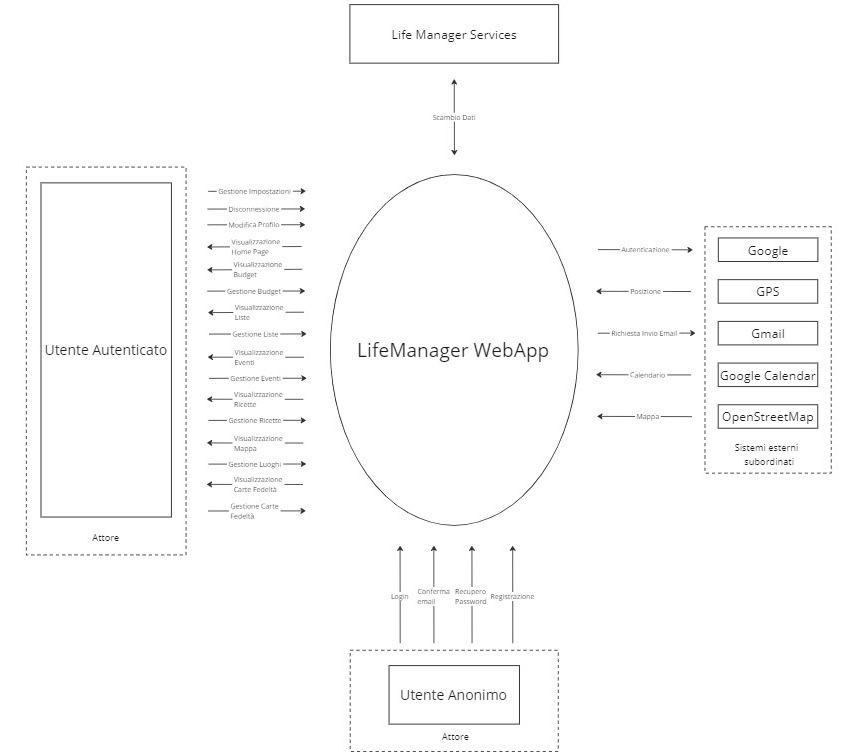
\includegraphics[width=15cm]{cd.jpg}
  \captionof{figure}{Context diagramma di LifeManager}
\end{center}

\begin{itemize} \setlength\itemsep{0.01em}
  \item{\sffamily  Utente non autenticato (anonimo)}
    \\L'utente non autenticato è l'attore qualsiasi che accede al sistema. Egli visualizza la pagina di Login in cui può scegliere se registrarsi (\hyperlink{RF1}{RF1}) o, se è già in possesso di un account, di effettuare l'accesso (\hyperlink{RF2}{RF2}). Registrazione e Login avvengono con le proprie credenziali personali o tramite il servizio offerto da Google (\hyperlink{RNF1}{RNF1}). L'utente anonimo, inoltre, può recuperare la propria password (\hyperlink{RNF2}{RNF2}).
    Dopo l'autenticazione, l'utente si specializza ''utente autenticato''.
    
    
 \item{\sffamily Utente autenticato}\\
    L'utente autenticato è colui che a seguito dell'autenticazione (\hyperlink{RF2}{RF2}) può fare il Logout, visualizzare i dati dell'account e modificarli, così come le impostazioni dell'applicativo. Inoltre vengono mostrate tutte le funzionalità dell'applicazione (\hyperlink{RF3}{RF3}) che egli può andare a svolgere (\hyperlink{RF4}{RF4}). 
   
   
  \item{\sffamily GPS}\\
    Il GPS è il sistema esterno subordinato che l'applicazione utilizza per ottenere le coordinate della posizione attuale (\hyperlink{RF19}{RF19}).
    
    
  \item{\sffamily Gmail}\\
    LifeManager utilizza il sistema esterno subordinato Gmail per inviare messaggi all'utente sotto forma di mail. Tali messaggi includono la conferma dell'account, il reset della propria password e le notifiche (\hyperlink{RF11}{RF11}, \hyperlink{RNF2}{RNF2}).
  
  
 \item {\sffamily Google}\\
    Google è il sistema esterno subordinato che LifeManager utilizza per accedere e registrarsi evitando la compilazione del modulo di registrazione (\hyperlink{RNF1}{RNF1}).  
 
 \item {\sffamily Google calendar}\\
    Nella sezione relativa agli eventi, l'utente visualizza un calendario fornito dal sistema esterno subordinato Google (\hyperlink{RF9}{RF9}). 
 
 \item {\sffamily OpenStreetMap}\\
    Il provider OpenStreetMap è il sistema esterno che viene usato per ottenere mappe da visualizzare in \hyperlink{RF16}{RF16}.

\item {\sffamily LifeManager services}\\
    LifeManager services è il sistema esterno paritario con cui LifeManager interagisce per ottenere, modificare, aggiungere dati al database. 

\end{itemize}

\vspace{0.5cm}
\hrule
\vspace{0.5cm}


Mauro Meneghello - mauro.meneghello@studenti.unitn.it

Luca Boschiero -  luca.boschiero@studenti.unitn.it

Nicola Turniano - nicola.turniano@studenti.unitn.it

%-----------------------------------------
 \end{document}